% CHAPITRE 5
\singlespacing
\chapter{Variation journalière de la respiration de l'écosystème (article)}
\label{ch:ch5}

\minitoc

\newpage

\doublespacing
\section{Introduction}
At a global scale, Ecosystem Respiration (ER) and photosynthesis are the most important fluxes between the atmosphere and the biosphere, accounting for 98 and 123 PgC yr $^{-1}$, respectively \citep{Bond-Lamberty2010,Beer2010}. 
By contrast the fossil fuel and cement production flux is one order of magnitude lower, at 7.8 PgC yr $^{-1}$ \citep{Ciais2014}.
Consequently, even small variations in the ecosystem fluxes may result in substantial changes in carbon (C) storage dynamics.
This can have a significant effect on the global C budget, in particular on atmospheric C concentration.
The C stock in natural ecosystems is divided into two pools: vegetation, which contains 450 to 650 Pg C, and the soil which contains 1500 to 2400 Pg C \citep{prentice2001,Eswaran1993,batjes1996}.
Across the world, the soil organic C (SOC) pool is spatially heterogeneous in terms of source and physical conditions, leading to variable storage rates between ecosystem types.
Peatlands are efficient C storage ecosystems.
They cover only 3\,\% of the global terrestrial area, but contain from 270 to 455 Pg C as SOC, i.e. from 10 to 30\,\% of the world's soil C \citep{gorham1991, turunen2002}.
Thus, peatlands are considered as a “hot spots” for SOC storage, and their evolution under current environmental changes deserves attention.

As in many other terrestrial ecosystems, many factors affect ER variability in peatlands: temperature, soil water content, vegetation, and substrate supply \citep{luo2006}.
All these factors are thought to be affected by global change, with unknown consequences on the C balance \citep{limpens2008}.
%Part of this uncertainty stems from the different formulations used to model the temperature sensitivity.
ER is often related to temperature: either to air temperature \citep[e.g.,][]{bortoluzzi2006}, or soil temperature.
%In the latter situation, different soil depths are used:
The most commonly used soil temperatures are those at -5 cm \citep{ballantyne2014,gorres2014} and -10 cm \citep{kim1992,zhu2015}.
%5 cm for \citet{Ballantyne2014,Gorres2014}, 10 cm for \citet{Kim1992,Zhu2015}.
In some studies, different depths are used and the selected one depends on the goodness-of-fit \citep{gunther2014, zhu2015}.
%Multiple depths are also used, the depth being chosen from the best goodness of fit \citep{Gunther2014, Zhu2015}.
All these studies use the chamber method to measure gas fluxes.
Even though most studies use -5 cm soil temperature, no clear consensus exists.
In addition \citet{pavelka2007} and \citet{graf2008} showed that the relationship between ER and temperature is depth dependent since heat transfer in the soil profile is not instantaneous and leads to a time-delay between the temperature and the ER signals.
%Time-delay might also lead to bias in Q$_{10}$ estimations which is widely use to describe the relationship between ER and the temperature despite its drawback \citep{Phillips2011, Davidson2006}.\textbf{(expliquer mieux avantages/inconvenients)}
The relationship between ER and temperature is often described using the Q$_{10}$ indicator, which represents the proportional increase of a reaction rate due to a 10\textdegree C rise in temperature.
However, even if the Q$_{10}$ seems coherent at a global scale \citep{mahecha2010}, reported values show a significant variability at the ecosystem level \citep{graf2008}.
Because the measured Q$_{10}$ are not linked to a single reaction but to multiple processes, numerous issues arise \citep{davidson2006}.
Among them are the time-scale considered \citep{curielyuste2004}, the depth \citep{graf2008} and the time-delays between ER and soil temperatures \citep{phillips2011}.
One way to deal with the time-delays might be data synchronisation according to \citet{pavelka2007}.
Another issue is the difference between the daytime and nighttime ER relationship with temperature. 
\citet{juszczak2012}, for example, showed that there are significant differences between ER modelled with daytime and nighttime data.
Assessing these differences may be important when working at a daily timescale and when treating data from eddy-covariance measurements.

Based on these previous studies, we expected that time-delays in \textit{Sphagnum}-dominated peatlands would be significant, even in the first 10 centimetres depth and that they would lead to a better description of observed data once taken into account, especially through data synchronisation.
To our knowledge no studies have explored the time-delay between ER and soil temperature in peatlands yet.
Differences in the ER--temperature relationship between daytime and nighttime datasets were also expected.
To test these predictions, ER fluxes, during the growing season in 4 \textit{Sphagnum}-dominated peatlands were measured in 2013.
Continuous measurements over 72 hours were carried out in each site using static dark chambers.
Air and soil temperature were also monitored.
Specifically, the relationship between ER and temperature, measured at different depths in peat was studied and the difference between daytime and nighttime measurements was assessed.

The aim of this study was (i) to highlight any time-delay at the daily timescale between ER and soil temperature at different depths in peatlands (ii) to assess the effect of synchronisation between ER and temperature in the representation of the diel ER variations (iii) to use the improved model to assess whether there is a difference between nighttime and daytime ER.

\subsection{Study sites}
The study was performed on four French \textit{Sphagnum}-dominated peatlands:
Bernadouze (BDZ, Ari\`ege; 3.75 ha, N 42\textdegree48’09”, E 1\textdegree25’24”, 1400 m), Frasne (FRN, Doubs; 98 ha, N 46\textdegree49’35”, E 6\textdegree10’20”, 836 m), Landemarais (LDM, Ille-et-vilaine; 23 ha, N 48\textdegree26’30”, E 1\textdegree10’54”, 154 m), and La Guette (LGT, Cher; 26 ha, N 47\textdegree19’44”, E 2\textdegree17’04”, 145 m).
%These sites compose the Peatland National Observatory System (certified by the CNRS/INSU).
Mean annual air temperatures and annual rainfalls were 6, 7.5, 11, 11\textdegree C, and 1700, 1400, 870, 880 mm for BDZ, FRN, LDM and LGT respectively.
During the measurements the water table level remained constant at to -12, -7, -35 and -9\,cm for BDZ, FRN, LDM and LGT.
%From this point they will be called BDZ (Bernadouze), FRN (Frasne), LGT (La Guette) and LDM (Landemarais).

\subsection{Data acquisition}
Fieldwork was conducted between July and October 2013. 
In each site, four plots (replicates) with similar plant cover were chosen.
Four cylindrical PVC collars (diameter: 31 cm, height: 15 cm) were inserted into the peat the day before beginning the measurements.
For 72 hours, CO$_{2}$ fluxes were measured in the 4 plots once an hour in random order.
These measurements were undertaken using a closed static chamber (diameter of 30.5 cm, height of 30 cm), with a GMP343 Vaisala probe.
ER was measured with a transparent chamber covered by an opaque material to avoid input of photosynthetic active radiation.
Inside the chamber the air was homogenized with a fan in order to minimize concentration gradients \citep{pumpanen2004}.
Measurement lasted a maximum of 5 min with CO$_{2}$ concentration recorded every 5 seconds as well as the relative humidity and the temperature inside the chamber.

In each site a weather station and a data logger were set up near the plots to provide meteorological and environmental data recorded every second: surface temperature (air temperature as close as possible to the surface: 5 cm), peat temperature (at -5, -10, -20 and -30 cm depth), air relative humidity and solar radiation. 
%These environmental parameters were recorded every second.

After the 72 hours of measurements four peat cores (30 cm height and 15 cm diameter), one for each replicate, were extracted at each site for physico-chemical characterisation.

\subsection{Data synchronisation}

The synchronisations between ER fluxes and temperatures were calculated for each depth and time-delays: 
% were then calculated.
%To avoid an artificial increase of data observations, no interpolations were made. (\textbf{clarifier phrase précédente})
The acquisition frequency between temperature and ER were different.
Thus an average of the temperatures recorded during the ER measurement time was calculated for all depths at the corresponding CO$_{2}$ flux measurement time.
%Then the temperature averaging procedure was repeated, with shifts of 10 minutes which is a compromise between precision and calculation time.
%This was performed up to 24 hours.
Then the temperature averaging procedure was repeated at 10-minute increments, until a 24 hour shift.
The 10-minute step was a compromise between precision and calculation time.
%With this procedure, the number of observation per site was constant.(\textbf{clarifier phrase précédente})
Next a correlation coefficient was calculated for each time step and temperature measurement depth.
Finally the synchronisation was determined for each depth, by selecting the time-delay corresponding to the highest correlation coefficient.
Negative correlations caused by the phase shift were discarded.

\subsection{Sensitivity of ER to temperature}
Three widely used models \citet{fang2001} were implemented to study the relationship between ER and temperature: Linear regression \eqref{eq_lin}, exponential models: Q$_{10}$ \eqref{eq_exp} and Arrhenius \eqref{eq_arr}
%Linear regression \eqref{eq_lin}, exponential models: Q$_{10}$ \eqref{eq_exp} and Arrhenius \eqref{eq_arr} model were implemented to study the relationship between ER and temperature as they are usually used \citet{fang2001}.
%, and \citet{Lloyd1994} \eqref{eq_lt} 
\begin{align}
ER & = \alpha + \beta T \label{eq_lin}\\
ER & = \alpha e^{\beta T} ; Q_{10}=e^{10*\beta} \label{eq_exp}\\
ER & = \alpha e^{\frac{-Ea}{RT}} \label{eq_arr}
%ER & = ae^{\frac{-b}{T-c}} \label{eq_lt}
\end{align}


%Linearization  was used over non-linear regression for robustness as measurements at daily scale leads to important ER variability relatively to the temperatures (Figure~\ref{fig:er_tair_tpeat}).
ER was estimated using air temperature, soil temperatures at -5, -10, -20 and -30 cm depth with both non-synchronised and synchronised datasets.
Calculations were implemented in R, and modelled data were adjusted to measured data using Ordinary Least Squares (OLS).
The goodness-of-fit was estimated by calculating the regression coefficient (R$^{2}$) and the root mean square error normalized by the mean (NRMSE).

\subsection{Testing difference between daytime and nighttime ER sensitivity to temperature}

To test whether the relationship between ER and temperature differed during daytime and nighttime, the dataset was split into two groups which were then compared.
The data between 10 am and 5 pm were considered as representative of the day and data between 11 pm and 6 am as representative of the night.
Only the air temperature and the -5 cm depth peat temperature (with synchronised and non-synchronised data) were investigated as they provide the best ER representation.
The data for day and night were centred to account for natural differences in measurement, since: during the day both temperature and ER are higher than in the night.
%Finally a paired student test was applied on the ratio between the centred ER and the centred temperature.
Using these centred data, ratios between ER and temperatures were calculated.
Finally a paired Student's t test was applied on the mean of the replicate for each site and each temperature to assess the significance of the differences between day and night measurements.

\subsection{Physico-chemical characterisation of the peat}

In the laboratory, two peat cores from each site were immersed in water during 24 hours to saturate the pores. 
Then, the cores were soaked overnight to get rid of the water filling the effective porosity. 
At 5 cm steps, a piece of peat with a known volume (V, cm$^{3}$) was cut and weighed (W1, g). 
Then, the samples were dried at 50\textdegree C for 48 hours and weighed (W2, g). 
Total porosity ($\Phi_{T}$, dimensionless), retention porosity ($\Phi_{R}$, dimensionless), effective porosity ($\Phi_{E}$, dimensionless) and bulk density (Bd, g cm$^{-3}$) were calculated as follows:

\begin{align}
\Phi_{T} & = 1 - \bigg[\frac{(\frac{W2}{\rho_{peat}})}{V}\bigg] \label{eq_por_tot}\\
\Phi_{R} & = 1 - \frac{\Big[\frac{(W1-W2)}{\rho_{peat}}\Big]}{V} \label{eq_por_ret}\\
\Phi_{E} & = \Phi_{T} - \Phi_{R} \label{eq_pro_eff}\\
Bd & = \frac{W2}{V} \label{eq_bd}
\end{align}

Peat density ($\rho_{peat}$) was set at 1.45 according to \citet{Kennedy2005}.
Then the peat was crushed and C, H, N and S analyses were performed with an elemental analyser (Thermo Flash analyser). 
%The pyrophosphate index (PPI), index of decomposition, was assessed at each depth by extracting 0.25 g of peat with 25 ml of a solution of pyrophosphate at 0.025 M (rotary shaker overnight), diluting the extract 10 times and measuring the absorbance at 550 nm with a spectrophotometer. 
%The PPI was calculated as follow:
%
%\begin{equation}
%PPI = Abs_{550} \times 100
%\end{equation}


\section{Results}

\subsection{Air temperature and ER variability}

Mean surface air temperatures were about 14-15\,\textdegree C for all sites, except for LGT which was 20.8 $\pm$ 7.4\,\textdegree C, (Figure~\ref{fig:er_tair_tpeat} -- H).
The lowest mean temperature and amplitude were found at BDZ: 14.4 $\pm$ 3.3\,\textdegree C (Figure~\ref{fig:er_tair_tpeat} -- E).
In LDM and FRN, the mean surface air temperatures were respectively 14.9 $\pm$ 8.7\,\textdegree C and 15.0 $\pm$ 10.3\,\textdegree C (Figure~\ref{fig:er_tair_tpeat} -- F, G)
Surface air temperature was the highest in FRN.
%FRN surface air temperature amplitude was the highest among all sites.
%Temperature range was the largest in FRN: 15.0 $\pm$ 10.4\,\textdegree C (Figure~\ref{fig:er_tair_tpeat} -- F).

At -5 cm depth, BDZ and LGT had lower mean temperatures than at the surface: 14.1 $\pm$ 1.5\,\textdegree C and 20.3 $\pm$ 1.7\,\textdegree C respectively, whereas the opposite was observed in FRN and LDM with 16.3 $\pm$ 2.4\,\textdegree C and 15.9 $\pm$ 1.0\,\textdegree C respectively.
Mean soil temperatures were still higher at -10 cm for both sites, but only in LDM at -20 cm.
At -30 cm the soil temperature amplitude ranged from 0.2 in LDM to 0.6 in LGT and FRN.
Overall conditions were warmer in LGT than in the other sites and LDM, despite a large amplitude of surface air temperature, had a particularly low soil temperature amplitude.

In terms of ER, mean and variability were the lowest in FRN among all sites (1.75 $\pm$ 0.83\,\textmu mol\,m$^{-2}$\,s$^{-1}$, Figure~\ref{fig:er_tair_tpeat} -- B).
%In contrary, FRN mean ER and variability were the lowest among all sites (1.75 $\pm$ 0.83\,\textmu mol\,m$^{-2}$\,s$^{-1}$, Figure~\ref{fig:er_tair_tpeat} -- B).
The highest variability and mean ER (6.13 $\pm$ 2.81\,\textmu mol\,m$^{-2}$\,s$^{-1}$, Figure~\ref{fig:er_tair_tpeat} -- C) were observed in LDM.
On this site replicates had different behaviours even though they were close to each other and in a similar environment.
%It is also in LDM where the ER variability was the highest.
In BDZ and LGT, ER mean values were 3.12 $\pm$ 0.92 and 4.10 $\pm$ 1.15\,\textmu mol\,m$^{-2}$\,s$^{-1}$ respectively (Figure~\ref{fig:er_tair_tpeat} -- A, B)

\begin{figure}
\centering
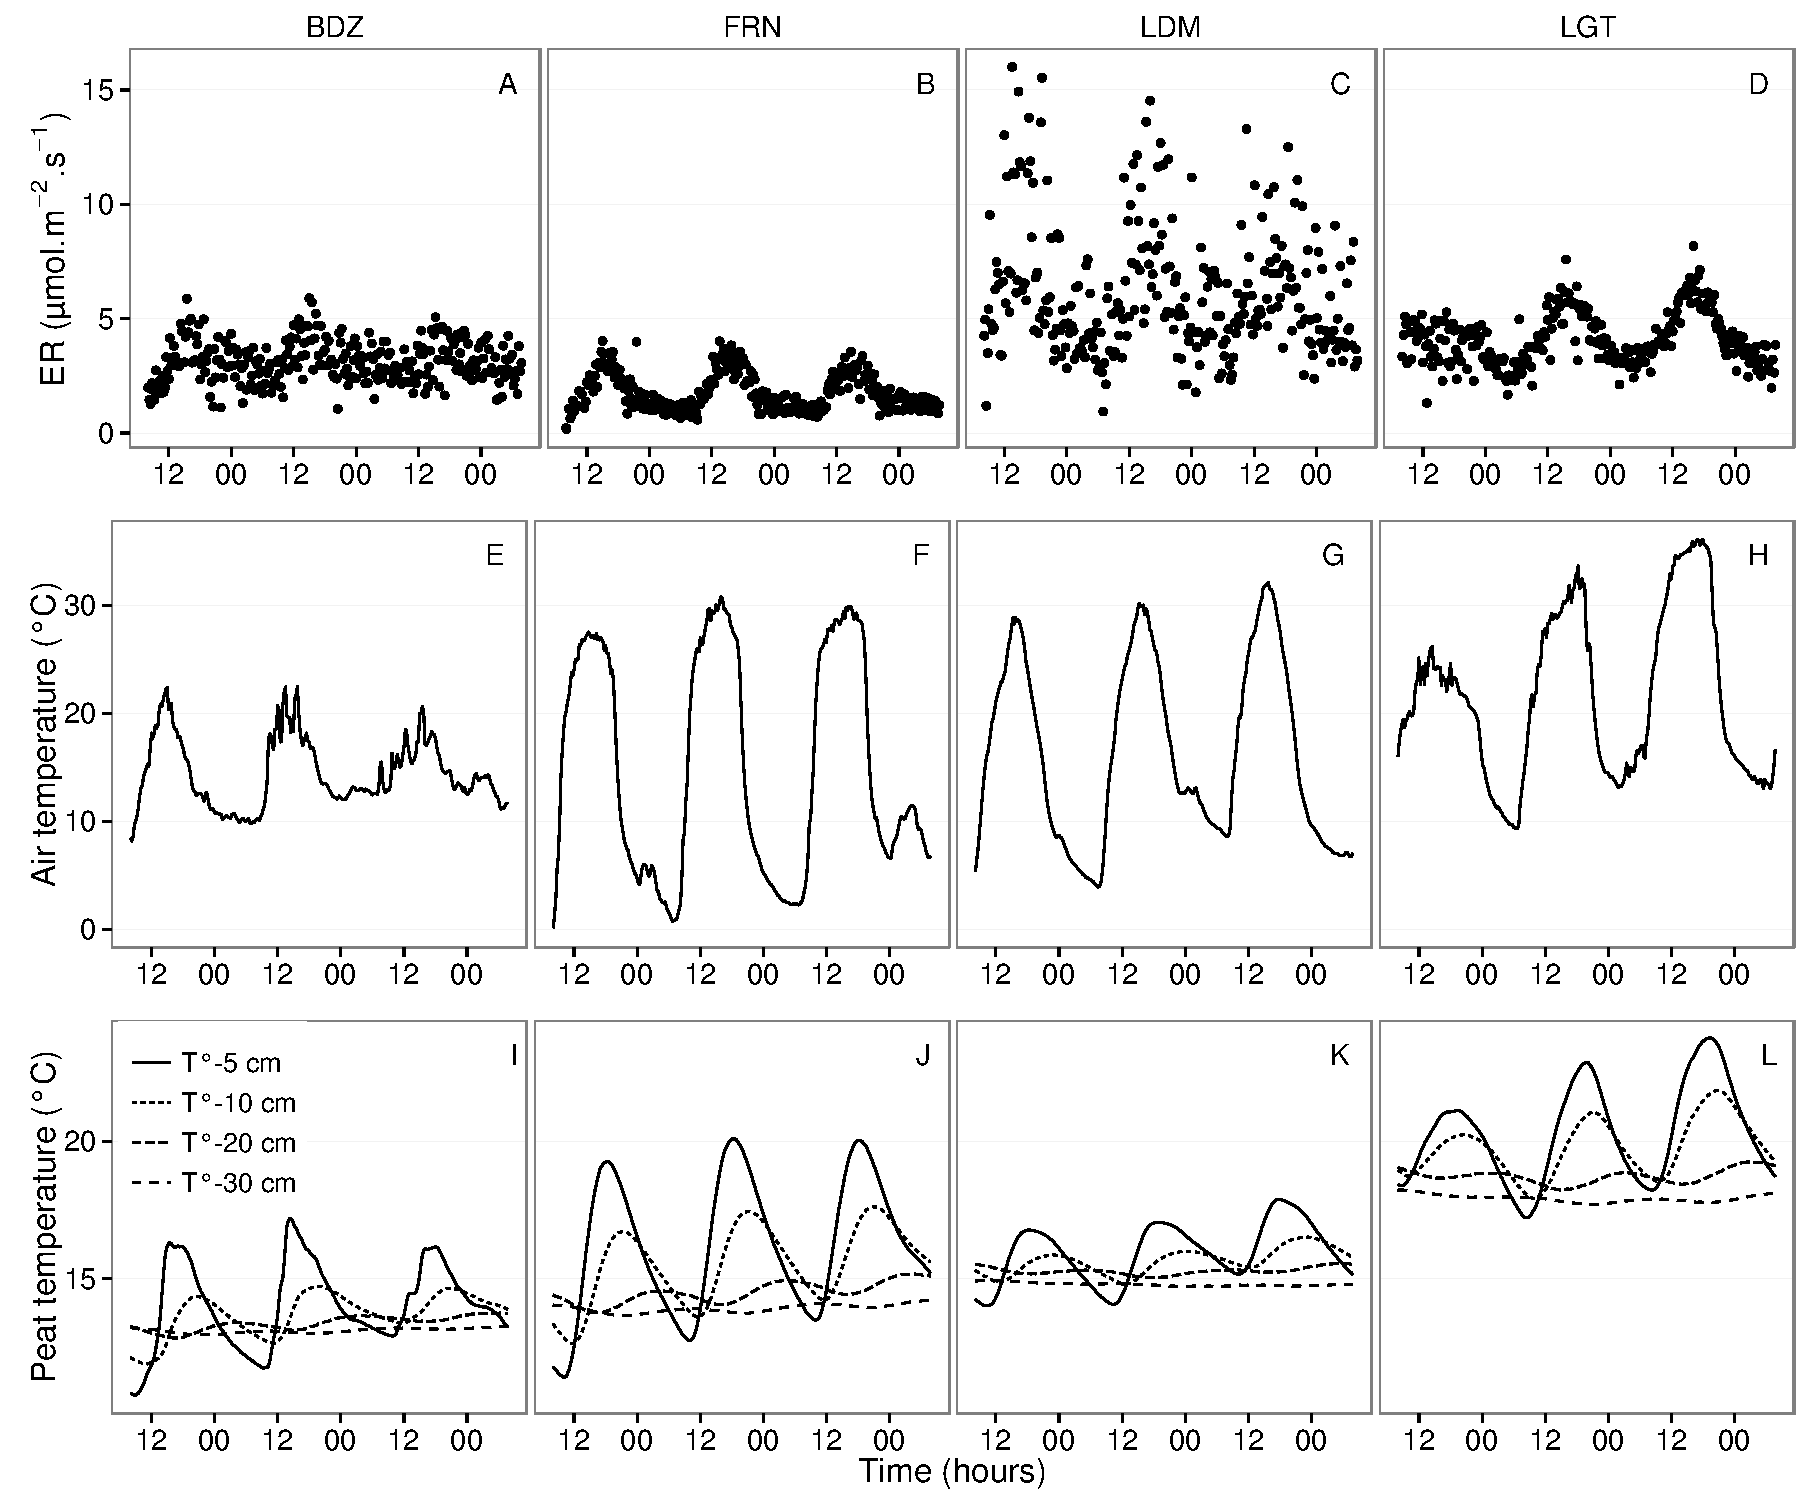
\includegraphics[width=\textwidth]{chap5/ER_Tair_Tpeat}
\caption{Ecosystem Respiration (ER), air and peat temperature, in the 4 sites (Bernadouze: BDZ, Frasne: FRN, Landemarais: LDM, La Guette: LGT).}
\label{fig:er_tair_tpeat}
\end{figure}

\subsection{ER and soil temperature synchronisation}
%\subsection{Synchronisation RE et température du sol}

Figure~\ref{fig:er_tair_tpeat} shows that the deeper the temperature was measured, the greater the shift with respect to ER.
Taking this shift into account by synchronising soil temperatures with ER led to a significant positive linear correlation between the temperature measurement depth and the synchronisation time-delay (all sites pooled, R$^2$=0.94, p$<$0.001; Figure~\ref{fig:lag_depth}).
The range of estimated time-delays decreased with depth up to -20 cm.
%At -20 cm, the time-delay in LDM was lower than the other three sites.
At this depth the time-delay was 12 hours, i.e. a phase inversion on a daily timescale.
For the three sites other than LDM, the slopes of the time-delay and measurement depth relationship were in a close range: 0.56, 0.54, 0.52 for FRN, BDZ and LGT respectively.
The relationship for LDM was higher at -30 cm, leading to a steeper slope (0.66) than in the other sites (Figure~\ref{fig:lag_depth}).
%In comparison with the other sites BDZ stood out with a lower time-delay at -5, whereas LDM have a higher one at -30 cm, leading to a higher slope than in the other sites: 0.66 (Figure~\ref{fig:lag_depth}).
At the other depths, this site always had the highest time-delay, though the values were close to those of the other sites.
BDZ always had the lowest time-delay, but like LDM, the values were close to those of the other sites, although slightly lower at -5 cm depth.

\begin{figure}[h]
\centering
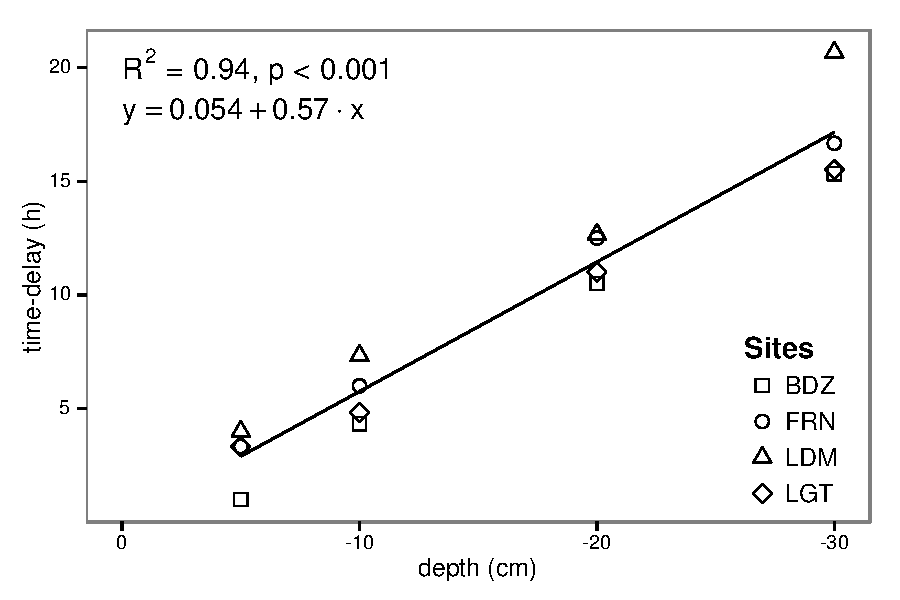
\includegraphics[width=.9\textwidth]{chap5/lag_depth}
\caption{Time delay between temperature at different depths and ER, in the 4 sites (Bernadouze: BDZ, Frasne: FRN, Landemarais: LDM, La Guette: LGT)}
\label{fig:lag_depth}
\end{figure}

\subsection{Model implementation}
%\subsection{Équations utilisées}

For both types of model (using non-synchronised and synchronised data), the differences between the 3 tested models were very small. 
The greatest differences, in R$^{2}$ values, were 0.07 and 0.05 for non-synchronised and synchronised data respectively, whereas differences in NRMSE maximum values were 1.28 and 1.14 (Table~\ref{table:mod_R2_RMSE}).
In most cases the linear model led to a slightly better R$^2$ than the others.
As the differences between equations were small, however, we will describe the exponential model in the following sections, because (i) it is the most widely used model to describe the ER--temperature relationship and (ii) the Q$_{10}$ value can be derived from this equation. 
This will allow the comparison of the results of our study to others.

%\newgeometry{left=1.5cm, right=1.5cm}
\begin{table}
\centering
\caption{R$^{2}$ and NRMSE profile with depth for models using non-synchronised and synchronised data and for the three equations (linear: lin, exponential: exp, arrhenius: arr).}
\hspace*{-1cm}
\begin{tabular}{lllllllllllll}
\hline
& \multicolumn{6}{l}{Non-synchronised} & \multicolumn{6}{l}{Synchronised} \\
 & lin &  & exp &  & arr & & lin &  & exp &  & arr &  \\[-.5ex] 
depth & R$^{2}$ & \textsc{nrmse} & R$^{2}$ & \textsc{nrmse} & R$^{2}$ & \textsc{nrmse} & R$^{2}$ & \textsc{nrmse} & R$^{2}$ & \textsc{nrmse} & R$^{2}$ & \textsc{nrmse} \\ 
\hline
\multicolumn{2}{l}{Bernadouze} & & & & & & & & & & & \\[-.5ex]
0 & 0.22 & 25.88 & 0.19 & 26.09 & 0.19 & 26.09 & 0.22 & 25.88 & 0.19 & 26.09 & 0.19 & 26.09\\
-5 & 0.23 & 25.66 & 0.20 & 25.89 & 0.20 & 25.89 & 0.27 & 25.18 & 0.24 & 25.40 & 0.24 & 25.40\\
-10 & 0.02 & 28.92 & 0.03 & 29.26 & 0.03 & 29.26 & 0.23 & 25.72 & 0.22 & 25.90 & 0.22 & 25.91\\
-20 & 0.04 & 28.64 & 0.03 & 28.98 & 0.03 & 28.98 & 0.13 & 27.79 & 0.13 & 28.16 & 0.13 & 28.15\\
-30 & 0.02 & 28.93 & 0.02 & 29.28 & 0.02 & 29.28 & 0.05 & 29.54 & 0.05 & 29.92 & 0.05 & 29.92\\
\multicolumn{2}{l}{Frasne} & & & & & & & & & & & \\[-.5ex]
0 & 0.66 & 27.58 & 0.63 & 26.74 & 0.63 & 26.96 & 0.66 & 27.58 & 0.63 & 26.74 & 0.63 & 26.96\\
-5 & 0.19 & 42.34 & 0.21 & 43.00 & 0.21 & 43.01 & 0.68 & 26.34 & 0.68 & 25.02 & 0.68 & 25.06\\
-10 & 0.01 & 46.73 & 0.00 & 48.01 & 0.00 & 48.01 & 0.59 & 29.98 & 0.60 & 29.20 & 0.60 & 29.22\\
-20 & 0.34 & 38.29 & 0.27 & 38.78 & 0.27 & 38.77 & 0.34 & 38.05 & 0.36 & 39.17 & 0.36 & 39.16\\
-30 & 0.03 & 46.30 & 0.03 & 47.47 & 0.03 & 47.47 & 0.18 & 43.66 & 0.19 & 44.75 & 0.19 & 44.74\\
\multicolumn{2}{l}{Landemarais} & & & & & & & & & & & \\[-.5ex]
0 & 0.29 & 38.55 & 0.32 & 39.31 & 0.32 & 39.24 & 0.29 & 38.55 & 0.32 & 39.31 & 0.32 & 39.24\\
-5 & 0.03 & 45.18 & 0.04 & 46.06 & 0.04 & 46.07 & 0.21 & 40.63 & 0.25 & 41.58 & 0.25 & 41.57\\
-10 & 0.05 & 44.53 & 0.04 & 45.45 & 0.04 & 45.45 & 0.13 & 42.65 & 0.16 & 43.71 & 0.16 & 43.7\\
-20 & 0.09 & 43.75 & 0.08 & 44.55 & 0.08 & 44.55 & 0.09 & 43.83 & 0.12 & 44.97 & 0.12 & 44.97\\
-30 & 0.03 & 45.09 & 0.02 & 46.07 & 0.02 & 46.07 & 0.13 & 44.94 & 0.12 & 46.02 & 0.12 & NA\\
\multicolumn{2}{l}{La Guette} & & & & & & & & & & & \\[-.5ex]
0 & 0.61 & 17.44 & 0.56 & 17.30 & 0.56 & 17.34 & 0.61 & 17.44 & 0.56 & 17.30 & 0.56 & 17.34\\
-5 & 0.31 & 23.27 & 0.29 & 23.24 & 0.28 & 23.26 & 0.63 & 16.83 & 0.59 & 16.49 & 0.58 & 16.51\\
-10 & 0.08 & 26.89 & 0.07 & 27.09 & 0.07 & 27.10 & 0.61 & 17.21 & 0.57 & 16.84 & 0.57 & 16.85\\
-20 & 0.30 & 23.41 & 0.27 & 23.30 & 0.27 & 23.30 & 0.54 & 18.93 & 0.51 & 19.01 & 0.51 & 19.01\\
-30 & 0.12 & 26.25 & 0.11 & 26.37 & 0.11 & 26.37 & 0.39 & 22.18 & 0.36 & 22.26 & 0.36 & 22.26\\
\hline
\end{tabular} 
\hspace*{-1cm}
%\belowtable{} % Table Footnotes\\
\label{table:mod_R2_RMSE}
\end{table}
%\restoregeometry

%\subsection{Relation entre RE et la température}
\subsection{ER and temperature relationship}

The relationship between air temperature and ER, using the exponential model, was better in LGT and FRN (R$^{2}$ $>$\,0.55) than in LDM and LDM (R$^{2}$ $<$\,0.35) (Table~\ref{table:mod_R2_RMSE}).
%For both linear and exponential model (\textbf{FIG4 and 5}), the relationship between air temperature and ER was better in LGT and FRN (R$^{2}$ ($>$\,0.6)) \textbf{(FL: LG < 0.6)} than in LDM and LDM (R$^{2}$ <\,0.4).
Nevertheless in all sites and with both linear and exponential models, using synchronised  soil temperatures gave a better account of the ER variability than their non-synchronised counterparts (Figure~\ref{fig:models_comparison}).
The goodness of fit (R$^2$) increased on average by 0.26 to 0.35 at -5 cm and -10 cm depth respectively.
The degree of improvement varied however between sites.
For instance, at -5 cm depth R$^2$ between synchronised and non-synchronised models increased by only 0.04 in BDZ while it increased by 0.47 in FRN.
The improvement gained by using synchronised data was higher at -5 cm and -10 cm than at deeper layers, with 0.12, 0.11 on average for -20 and -30 cm depth (Figure~\ref{fig:models_comparison}).
%The improvement gained by using synchronised data was lower, deeper in the profile: 0.12, 0.11 on average for -20 and -30 cm depth.

A similar observation can be made for NRMSE.
Regardless of some exceptions at deeper layers especially at -20 cm depth, the NRMSE values show that using synchronised data rather than non-synchronised ones improved the representation of ER variability at a daily timescale, indicating that depth measurements dependence is smaller for models using synchronised data than for models using non-synchronised data.
However with increasing depth R$^{2}$ values still decreased and NRMSE values still increased.
For FRN, LDM and LGT, synchronised data at -5 cm depth gave a better account of the ER variability than surface air temperature (Figure~\ref{fig:models_comparison}).
This was not the case in LDM, where temperature at the surface was the best descriptor of ER.
For both R$^{2}$ and NRMSE the values at -20 cm depth were better than those observed at -10 or -30 cm depth.
This pattern was observed with different magnitudes among sites, and was particularly visible in FRN and LGT.
For the most part, the synchronisation of data led to higher R$^{2}$ and NRMSE values for models using one soil temperature, at a daily scale on \textit{sphagnum}-dominated peatlands.

\begin{figure}[]
\centering
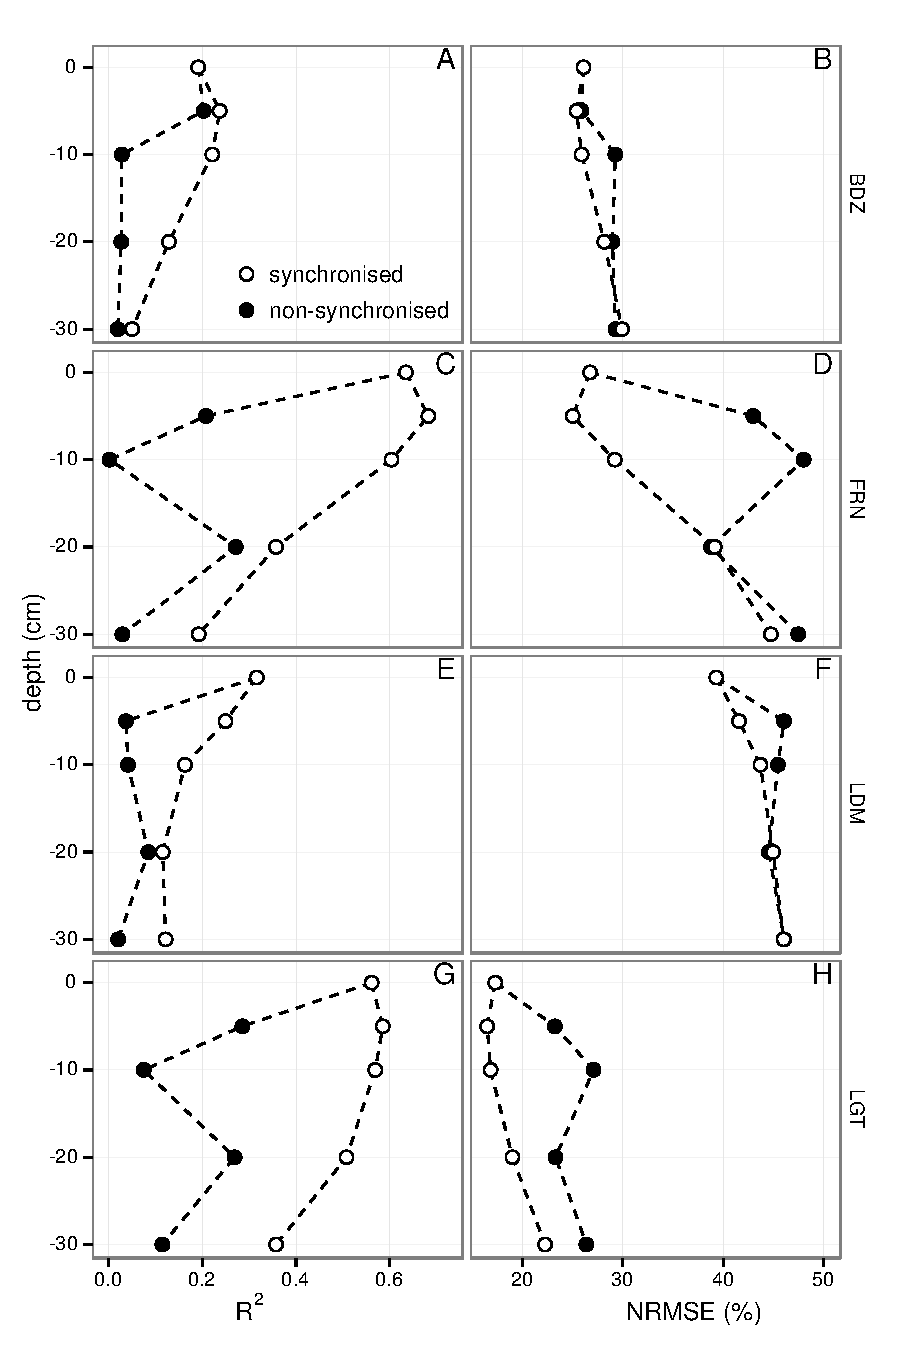
\includegraphics[width=\textwidth]{chap5/oneT_indic}
\caption{Profile of R$^{2}$ and NRMSE, (RMSE, normalized by the mean), with depth, in the 4 sites (Bernadouze: BDZ, Frasne: FRN, Landemarais: LDM, La Guette: LGT) using the exponential model.}
\label{fig:models_comparison}
\end{figure}

%\subsection{Évolution du Q10}
\subsection{Q$_{10}$ evolution}

The Q$_{10}$ stood between 0 and 2.5 for non-synchronised data with a maximum at -5 cm depth.
Average values were 1.4, 2.4 and 1.3, at the surface, -5 and -10 cm depth respectively (Figure~\ref{fig:oneT_Q10}).
Average Q$_{10}$ values at the surface and -10 cm depth were very similar.
However there was much more variability at -10 cm depth, where the values ranged from 0.1 to 2.1, than at the surface where the values stood between 1.3 and 1.5.
%Although values at 0 and -10 cm depth are close, there is much more variability in the latter than in the former as the values range from 0.1 to 2.1.
Beyond -10 cm depth Q$_{10}$ values fell almost to 0, while for non-synchronised data Q$_{10}$ values greatly increased with depth, reaching meaningless values.
Q$_{10}$ values estimated with surface temperature were very similar between sites with an average of 1.4 (Figure~\ref{fig:oneT_Q10}).
It increased to about 2.5 at -5 cm depth, with both synchronised and non-synchronised data.
Below this depth, Q$_{10}$ estimated with both methods either decreased downwards (non-synchronised) or increased (synchronised data) to unrealistic values (Figure~\ref{fig:oneT_Q10}).

\begin{figure}
\centering
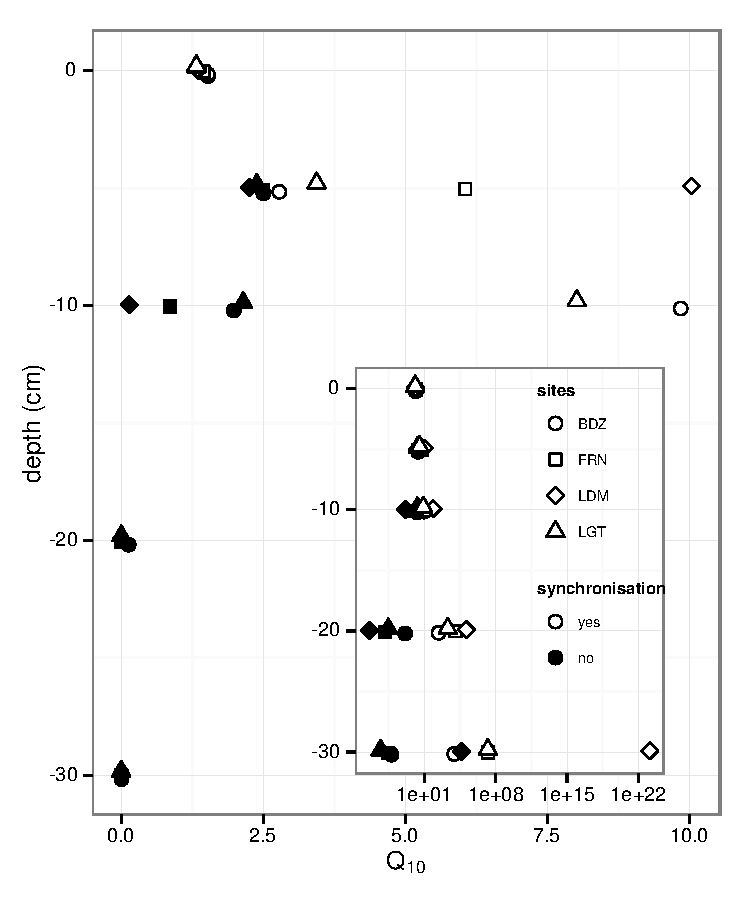
\includegraphics[width=\textwidth]{chap5/oneT_Q10}
\caption{Profile of Q$_{10}$ with depth for synchronised (white) and non synchronised (black) data and exponential model in the 4 sites (Bernadouze: BDZ, Frasne: FRN, Landemarais: LDM, La Guette: LGT).}.
\label{fig:oneT_Q10}
\end{figure}
%\textbf{CG: Mentionner ce qu'est une valeur réaliste du Q10 (entre 1.5 et 2.5 si je me souviens bien, en s'appuyant sur des références), texte mieux dit en dessous}

%\subsection{Différence entre mesures de jour et de nuit}
\subsection{Daytime and nighttime differences}


For BDZ and LDM sites no significant differences were found between daytime and nighttime data no matter which model was used, whereas differences were found for FRN and LGT (Figure~\ref{fig:diff_JN}). 
In FRN, synchronisation increased the significance of the differences: p $<$ 0.001 with and p $<$ 0.01 without synchronisation respectively.
The same pattern was found in LGT but with lower significance.
Hence models using -5 cm depth with non-synchronised data are not significantly different but those using synchronised data are.
%Note that, for LGT, the model using synchronised data with -5 cm depth temperature and the model using air temperature do not show the same differences:
Note that, for LGT, the model using air temperature had a daytime slope that was higher than the nighttime one, which was the opposite of all the other cases.
% do not show the same difference between daytime and nighttime.
%Daytime slope are superior to nighttime ones for the former as are all the other differences and inferior for the latter.

\begin{figure}
\centering
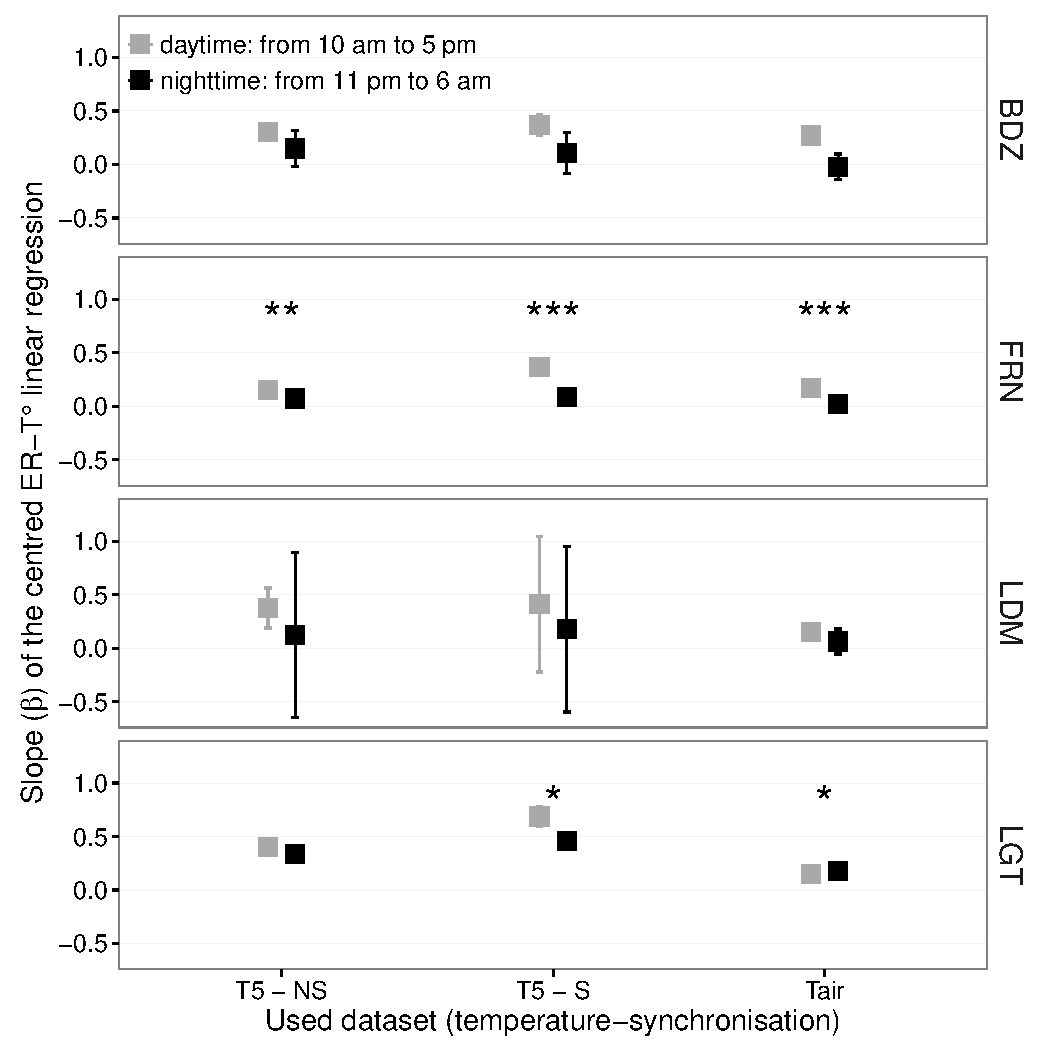
\includegraphics[width=\textwidth]{chap5/diff_JN_lin}
\caption{Differences between daytime and nighttime measurements using 3 models: non-synchronised data at -5 cm depth temperature (T5 -- NS), synchronised data at -5 cm depth temperature (T5 -- S), and non-synchronised data at air temperature (Tair).}
\label{fig:diff_JN}
\end{figure}

%\subsection{Caractérisation de la tourbe}
\subsection{Peat characterisation}

%Peat from LGT was the most decomposed among the studied sites as shown by the increasing PPI with depth, with a maximum, above 90, in the 20-25 cm section (Table~\ref{table:phychi}).
%By contrast, the least decomposed peat was from FRN with a PPI inferior to 4 at any depth.
Elemental compositions were similar in all sites: 1--3\%, 4--6\% and $<$1\% for N, H and S respectively (Table~\ref{table:phychi}).
C content was mainly between 40 and 50 \%, except at the deeper levels in LDM and LGT where values were lower ($<$ 32\%).

\begin{table}
\centering
\caption{Peat chemical properties as a function of depth in cm: content (\%) N, C, H, S, the total, retention and effective porosity, $\Phi_{T}$, $\Phi_{R}$, $\Phi_{E}$ respectively in $m^{3}.m^{-3}$, solid peat volumic fraction in $m^{3}.m^{-3}$ and the bulk density (Bd) in $g.cm^{-3}$.} 
\begin{tabular}{llllllllll}
\toprule
% & & & & & & & \multicolumn{3}{c}{Porosity} & \\
%level (cm) & N (\%)& C (\%)& H (\%)& S (\%)& PPI & $\Phi_{T}$ & $\Phi_{R}$ & $\Phi_{E}$ & solid & Bd \\
level  & N & C & H & S & $\Phi_{T}$ & $\Phi_{R}$ & $\Phi_{E}$ & solid & Bd \\
%(cm) & (\%) & (\%)& (\%)& (\%)&  & $m^{3}.m^{-3}$ & porosity & porosity & & density\\
\midrule
\multicolumn{2}{l}{Bernadouze} & & & & & & & & \\[-.5ex] 
0--5 & 1.76 & 41.84 & 6.05 & 0.05   & 0.99 & 0.47 & 0.52 & 0.01 & 0.03 \\
5--10 & 1.99 & 43.99 & 6.18 & 0.07 & 0.97 & 0.78 & 0.19 & 0.03 & 0.06 \\
10--15 & 2.28 & 45.38 & 6.35 & 0.10 & 0.96 & 0.92 & 0.04 & 0.04 & 0.10 \\ 
15--20 & 2.92 & 44.95 & 6.23 & 0.23 & 0.95 & 0.82 & 0.13 & 0.05 & 0.11 \\ 
20--25 & 3.14 & 39.01 & 5.31 & 0.23 & 0.93 & 0.90 & 0.04 & 0.07 & 0.16 \\
25--30 & 2.50 & 31.15 & 4.28 & 0.13 & 0.89 & 0.86 & 0.03 & 0.11 & 0.24 \\
\multicolumn{2}{l}{Frasne} & & & &  & & & & \\[-.5ex] 
0--5 & 1.73 & 43.67 & 6.24 & 0.00 & 0.99 & 0.40 & 0.58 & 0.01 & 0.03 \\ 
5--10 & 1.55 & 43.35 & 5.97 & 0.00 & 0.98 & 0.59 & 0.40 & 0.02 & 0.03 \\
10--15 & 1.69 & 43.49 & 6.17 & 0.00 & 0.98 & 0.89 & 0.09 & 0.02 & 0.05 \\
15--20 & 1.63 & 43.06 & 5.97 & 0.00 & 0.98 & 0.89 & 0.09 & 0.02 & 0.05 \\
20--25 & 1.30 & 43.68 & 6.29 & 0.05 & 0.98 & 0.93 & 0.04 & 0.02 & 0.05 \\ 
25--30 & 1.48 & 43.44 & 6.21 & 0.03 & 0.98 & 0.87 & 0.11 & 0.02 & 0.05 \\
\multicolumn{2}{l}{Landemarais} & & & & & & & & \\[-.5ex] 
0--5 & 1.36 & 45.63 & 5.69 & 0.25 & 0.97 & 0.62 & 0.35 & 0.03 & 0.07 \\
5--10 & 3.08 & 47.37 & 5.37 & 0.09 & 0.95 & 0.74 & 0.21 & 0.05 & 0.11 \\
10--15 & 2.73 & 48.34 & 5.63 & 0.10 & 0.94 & 0.94 & 0.00 & 0.06 & 0.13 \\
15--20 & 2.54 & 48.67 & 5.64 & 0.30 & 0.96 & 0.81 & 0.15 & 0.04 & 0.10 \\
20--25 & 2.08 & 46.99 & 5.80 & 0.23 & 0.97 & 0.89 & 0.08 & 0.03 & 0.07 \\
25--30 & 1.57 & 45.65 & 6.23 & 0.21 & 0.97 & 0.89 & 0.08 & 0.03 & 0.07 \\
\multicolumn{2}{l}{La Guette} & & & & & & & & \\[-.5ex] 
0--5 & 1.55 & 38.33 & 5.23 & 0.05 & 0.97 & 0.61 & 0.36 & 0.03 & 0.05 \\
5--10 & 2.35 & 41.31 & 4.66 & 0.20 & 0.93 & 0.83 & 0.10 & 0.07 & 0.08 \\
10--15 & 2.34 & 43.81 & 5.72 & 0.18 & 0.91 & 0.89 & 0.02 & 0.09 & 0.10 \\
15--20 & 1.99 & 43.17 & 5.45 & 0.10 & 0.89 & 0.87 & 0.01 & 0.11 & 0.13 \\
20--25 & 1.90 & 37.91 & 4.83 & 0.05 & 0.88 & 0.83 & 0.05 & 0.12 & 0.15 \\ 
25--30 & 1.32 & 18.95 & 2.32 & 0.01 & 0.79 & 0.76 & 0.03 & 0.21 & 0.28 \\
\bottomrule
\end{tabular}
%\belowtable{} % Table Footnotes
\label{table:phychi}
\end{table}

%\section{Discussion}
%
%\subsection{Différence de RE entre les différents sites}
\section{Discussion}

\subsection{ER differences between sites}


The ER fluxes calculated in the 4 sites were in the same order of magnitude as those of peatlands found in the literature.
\citet{bortoluzzi2006}, for instance, found ER values ranging from 2 to 5\, during the same period as this study, i.e. July to October 2004.
In the present study, the models performed poorly in 2 sites, BDZ and LDM.
For BDZ, amplitudes of both ER and temperatures were low  (Figure~\ref{fig:er_tair_tpeat} -- A, E) making the representation of ER possible only on a short temperature span.
With such low ranges of both ER and temperature, it can be assumed that ER variability was due to the variability between plots.
% and the noise more preponderant.
For LDM, the ER fluxes were measured in plots that were more heterogeneous than expected, resulting in strong variability (Figure~\ref{fig:er_tair_tpeat} -- C).
%Actually the replicates can be grouped 2 by 2, one group showing ER values close to XXXX data and the other :XXXX.
This observation is consistent with the high NRMSE value calculated for this site (39.3 \% for BDZ against 26.1 \% for LDM) whereas the R$^{2}$ values for these two sites were close, 0.19 and 0.32 for BDZ and LDM respectively, using surface air temperature and an exponential relationship.
It is noteworthy that in FRN the NRMSE values were high with respect to R$^{2}$ values.
%It is noteworthy that in FRN the NRMSE values were higher than in the other sites.
This result can be explained by the fact that the mean ER flux was low (1.75\,\textmu mol\,m$^{-2}$\,s$^{-1}$) and thus had a strong influence on NRMSE as we used mean normalization.
Finally at -20 cm depth, models using non-synchronised data showed, an increase in R$^{2}$ and a decrease in NRMSE which was more or less observable in the different sites:
clearly in FRN, LGT and to a lesser extent in LDM, but barely perceivable in BDZ.
At this depth the temperature and the ER signal phases are opposed making the non-synchronised models better at representing ER than at -10 or -30 centimetres but with a reverse relationship.
The ER fluxes thus show different behaviours either in their amplitude or in their homogeneity

%\subsection{Temps de latence entre température et RE}
\subsection{Time-delay between temperature and ER}

Time-delays between soil temperatures and ER occur in \textit{Sphagnum}-dominated peatlands.
They occur even close to the soil surface and increase with depth.
The relationship between time-delays and depth was similar in all the studied sites although LDM had slightly higher time-delays.
The overall delay observed in peat soils, 0.57 hours per centimetre, was higher than those found by \citet{pavelka2007} in a forest and in a grassland ecosystem and by \citet{parkin2003} on two agricultural soils (0.4 and 0.5 hours per centimetre respectively).
This is coherent with the fact that peat soil has a lower thermal diffusivity than mineral soils \citep{farouki1981,arya2001}.
LDM was the only site with a slightly higher slope especially at -30 cm.
This was expected as soil diffusivity increases with wetness \citep{hillel2003} and LDM was the site with the lowest water table level.
This was confirmed by thermal conductivity measurements conducted on the peat cores (data not shown).
%BDZ is the only site which is regularly grazed by cows. 
%Therefore, one hypothesis to explain the low time-delay recorded at -5 cm depth is the resulting soil compaction. 
%Indeed \citet{Lipiec2003} report that increases in soil compaction lead to higher thermal conductivity and thus to a lower time-delay.
%An other hypothesis is the temperature probe position as it is difficult to place it precisely particularly at shallow depth.
%Overall even with sites with different behaviour in term of ER fluxes the time-delays are similar in all sites
Overall, it should be noted that the time-delays were similar in all the studied sites despite their variability in terms of ER fluxes.

%\subsection{La synchronisation entre RE et la température améliore la représentation de la sensibilité de RE à la température}
\subsection{Synchronising ER and temperature improves ER sensitivity to temperature representation}

In spite of the importance of lags between physical phenomenona and biological activities \citep{vargas2010}, few studies have addressed the effect of time-delays between soil temperature and global biological activity (ER) at the daily timescale.
At this scale, we showed in peatlands that using synchronised data improved the representation of the temperature sensitivity of ER.
The improvement provided by synchronisation was evidenced at shallow depth.
The best goodness-of-fit obtained with synchronised data and models using one temperature, was found at -5 cm depth.
These observations are in agreement with those of \citet{pavelka2007} who also found a decreasing effect of synchronisation with depth.
Such a lesser depth effect could be explained by a simultaneous decrease in temperature amplitude.
Because the goodness-of-fit of the non-synchronised data increases at -20 cm, the synchronisation effect  strongly decreases at this depth.
This pattern is visible, with various amplitudes, in the different sites.
It is explained by the 12 h time-delay (Figure~\ref{fig:lag_depth}) corresponding to a phase inversion that occurs at this depth between the ER and the daily temperature courses.
Such a phase inversion was found deeper, at -30 cm by \citet{pavelka2007}, due to a higher temperature diffusivity in mineral soils.
Finally in our study these models, using synchronised -5 cm depth temperature, show slightly higher R$^2$ and lower NRMSE values than those using surface air temperature.
%Our results showed that in most cases, soil temperature is a better predictor than air temperature and should be used instead.

%\subsection{Différence entre mesure de RE faite le jour et la nuit}
\subsection{Differences between daytime and nighttime ER measurements}

The significant differences observed between daytime and nighttime measurements corroborate other studies in which these differences were found using chamber techniques \citep{juszczak2012,darenova2014}.
The fact that some sites show significant differences (FRN and LGT) and not others (BDZ and LDM) seems to be linked to the variability between plots and temperature amplitude.
When temperature amplitude was low, most of the variability originated from spatial variability between plots.
%the noise in the data: less noise, higher significance and high noise lower or no significance.
This was also corroborated by a test done on LGT where we calculated the day and night differences only on the last two days when temperature amplitude was the greatest.
%thus avoiding the first noisy day.
As a result the significance increased from p\,$<$\,0.05 to p\,$<$\,0.01 for the synchronised model using -5 cm depth temperature and the differences observed in the model using air temperature were no longer significant any more (p\,$>$\,0.05).


%\subsection{La sensibilité du Q10 à la profondeur de la température et à la synchronisation}
\subsection{Q$_{10}$ sensitivity to temperature depth and synchronisation}

In shallow layers ($\leq$ 10 cm), the Q$_{10}$ values calculated with non-synchronised data in the ranges that are usually reported, i.e. between 1.3 to 3.3 \citep{raich1992}.
At deeper levels in the peat profile ($\geq$ 10 cm), they reach 0 as the relationship between ER and the temperature weakens, and is not compensated by a long term evolution.
A similar behaviour was found by \citet{pavelka2007} even if this Q$_{10}$ decrease with depth is not usually seen and most studies show the opposite, namely an increase in Q$_{10}$ values with depth \citep{graf2008}.
This apparent contradiction may be explained by the length of the study.
%Because of the short duration of the study, the effect of the time-delays on the relationship between ER and the temperatures are preponderant over the relation itself.
Because of its short duration, the effect of the time-delays on ER were preponderant over the temperature effect.
Synchronisation also led to meaningless high Q$_{10}$ values because synchronisation can explain a higher proportion of ER flux with a smaller temperature variation.
Temperature amplitude decreases with depth because of soil dampening.


\section{Conclusions}  %% \conclusions[modified heading if necessary]

We showed that the time-delays between ER and soil temperatures at different depths are significant on a daily timescale as the signals are shifted 30 minutes every centimetre.
At this scale the  use of synchronised soil temperature, to take into account these time-delays, can improve the representation of ER particularly in the first 10 centimetres.
Only one of the studied sites showed highly significant differences between daytime and nighttime measurements.
However it is possible that such differences exist in the other sites, depending on the environmental conditions (e.g. temperature amplitude) and spatial variability in the ER fluxes.
Addressing questions of bio-physical coupling in determining ER at different timescales requires high frequency observations \citep{Vargas2011}.
Even if the automated chamber technique is increasingly used, it cannot be easily deployed in some sites due to tall vegetation, power supply difficulties, or harsh environmental conditions.
In contrast, temperature measurements at different depths are easy to conduct, robust to harsh conditions and can be powered by a small solar panel.
A calibration campaign with human manipulated closed chambers could be carried out to assess ER variability at different timescales.
Coupling temperature profile and punctual ER measurements and then using synchronised data in models may be a good alternative in sites where automated chambers are not easily implantable.

\section*{Acknowledgements}
The work was funded as part of the Peatland National Observatory Service (Service national d'observation Tourbi\`eres, certified by the CNRS/INSU) as the four studied sites are part of this Service. The authors are also indebted to the site managers for permitting access to the studied peatlands. We also acknowledge support from Labex VOLTAIRE (ANR-10-LABX-100-01). Finally we would like to thank Elizabeth Rowley-Jolivet for corrections to the manuscript.